\section{Auswertung}
\label{sec:Auswertung}

\begin{table}[H]
  \centering
  \caption{Messdaten zur Nullmessung beim $\gamma$-Zerfall.}
  \label{tab:Zerfall0}
  \sisetup{table-format=3.0}
  \begin{tabular}{S S @{${}\pm{}$}S[table-format=2.2] S[table-format=1.2] @{${}\pm{}$}S[table-format=1.2] }
    \toprule
  \multicolumn{1}{p{2cm}} {Messzeit $t / \si{\second}$} & \multicolumn{2}{c}{$N$}& \multicolumn{2}{c}{$\frac{N}{t} / \frac{1}{\si{\second}}$}\\
    \midrule
    900 & 828 & 28.77 & 0.92 & 0.03\\
  \bottomrule
  \end{tabular}
\end{table}


\begin{table}[H]
  \centering
  \caption{Messdaten zum $\gamma$-Zerfall mit Eisen als Absorber.}
  \label{tab:gammaEisen}
  \sisetup{table-format=2.2}
  \begin{tabular}{S[table-format=2.1] S[table-format=2.0] S[table-format=4.0]@{${}\pm{}$} S[table-format=2.2] S[table-format=3.2] @{${}\pm{}$}S[table-format=1.2]}
    \toprule
    \multicolumn{1}{p{2cm}}{ $ d/ \si{\milli\meter}$} &\multicolumn{1}{p{2cm}} {Messzeit $t / \si{\second}$} & \multicolumn{2}{c}{$N$}& \multicolumn{2}{c}{$\frac{N}{t} / \frac{1}{\si{\second}}$}\\
    \midrule
       0.0 &  60 &  6976 & 83.52 & 116.27 & 1.39 \\
       0.5 &  60 &  6738 & 82.09 & 112.30 & 1.37 \\
       1.0 &  60 &  6635 & 81.46 & 110.58 & 1.36 \\
       1.5 &  60 &  6374 & 79.84 & 106.23 & 1.33 \\
       2.0 &  60 &  6463 & 80.39 & 107.72 & 1.34 \\
       2.5 &  60 &  6261 & 79.13 & 104.35 & 1.32 \\
       3.0 &  60 &  5622 & 74.98 &  97.30 & 1.25 \\
       5.0 &  60 &  5410 & 73.55 &  90.17 & 1.23 \\
       6.0 &  60 &  5681 & 75.37 &  94.68 & 1.26 \\
       7.0 &  60 &  5318 & 72.92 &  88.63 & 1.22 \\
      10.0 &  60 &  4569 & 67.59 &  76.15 & 1.13 \\
      15.0 &  60 &  4101 & 64.04 &  68.35 & 1.07 \\
      20.0 &  60 &  2955 & 54.36 &  49.25 & 0.91 \\
      25.0 &  60 &  2428 & 49.27 &  40.47 & 0.82 \\
  \bottomrule
  \end{tabular}
\end{table}

\begin{table}[H]
  \centering
  \caption{Messdaten zum $\gamma$-Zerfall mit Blei als Absorber.}
  \label{tab:gammaBlei}
  \sisetup{table-format=2.2}
  \begin{tabular}{S[table-format=2.1] S[table-format=2.0] S[table-format=4.0]@{${}\pm{}$} S[table-format=2.2] S[table-format=3.2] @{${}\pm{}$}S[table-format=1.2]}
    \toprule
    \multicolumn{1}{p{2cm}}{ $ d/ \si{\milli\meter}$} &\multicolumn{1}{p{2cm}} {Messzeit $t / \si{\second}$} & \multicolumn{2}{c}{$N$}& \multicolumn{2}{c}{$\frac{N}{t} / \frac{1}{\si{\second}}$}\\ 
       0.0 &  60 & 6718 & 81.96 & 111.97 & 1.37 \\
       1.0 &  60 & 5866 & 76.59 &  97.77 & 1.28 \\
       2.0 &  90 & 7875 & 88.74 &  87.50 & 0.99 \\
       3.0 &  90 & 7675 & 87.61 &  85.28 & 0.97 \\
       4.0 &  90 & 6727 & 82.02 &  74.74 & 0.91 \\
       5.0 &  90 & 5963 & 77.22 &  66.26 & 0.86 \\
       6.0 &  90 & 5287 & 72.71 &  58.74 & 0.81 \\
      10.0 & 120 & 5014 & 70.81 &  41.78 & 0.59 \\
      11.0 & 150 & 5913 & 76.90 &  39.42 & 0.51 \\
      12.0 & 150 & 5363 & 73.23 &  35.75 & 0.49 \\
      14.0 & 180 & 5103 & 71.44 &  28.35 & 0.40 \\
      15.0 & 180 & 4511 & 67.16 &  25.06 & 0.37 \\
  \bottomrule
  \end{tabular}
\end{table}

Aus den Messwerten wird die Aktivität 
\begin{align}
  A= \frac{N}{t}-\frac{N_0}{t}
\end{align}
berechnet.
Diese wird logarithmisch in Beziehung zur Schichtdicke $d$ in \autoref{fig:plot1} beziehungsweise \autoref{}

\begin{figure}[H]
  \begin{subfigure}{\textwidth}
    \centering
    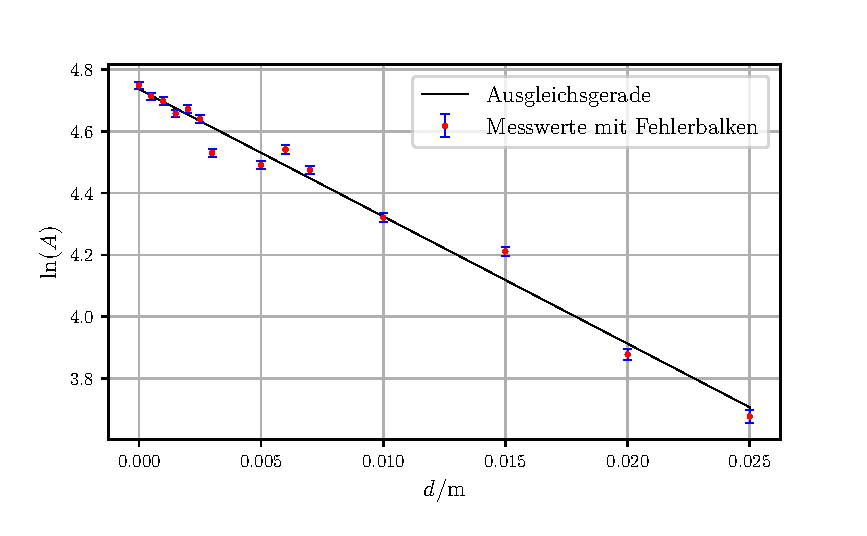
\includegraphics[scale=0.75]{build/plot1.pdf}
    \caption {Lineare Ausgleichsrechung zur Bestimmung des Absorptionskoeffizienten
    $\mu_{\text{Fe}}$ von Eisen.}
    \label{fig:plot1}
  \end{subfigure}
  \hfill
  \begin{subfigure}{\textwidth}
    \centering
    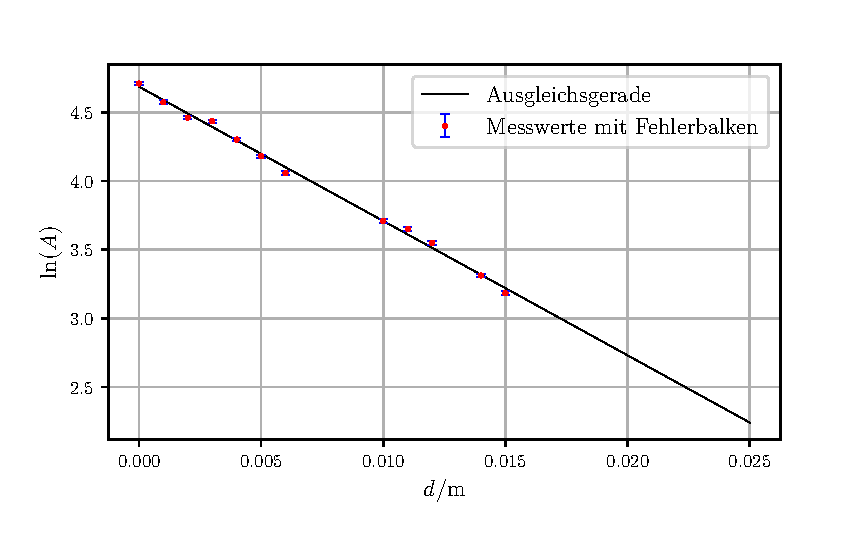
\includegraphics[scale=0.75]{build/plot2.pdf}
    \caption {Lineare Ausgleichsrechung zur Bestimmung des Absorptionskoeffizienten
    $\mu_{\text{Pb}}$ von Blei.}
    \label{fig:plot2}
  \end{subfigure}
    \caption {Messdaten zur Bestimmung der Absorptionskoeffizienten aus der Zählrate.}
  \end{figure}


